
In Figure \ref{fig:myGIARates}, the values for relative GIA produced by this paper are
visualized by plotting the absolute value range of GIA rates between each site
as a line between sites on the map with the corresponding value next to it.

\begin{figure}[h]
	\makebox[\textwidth]{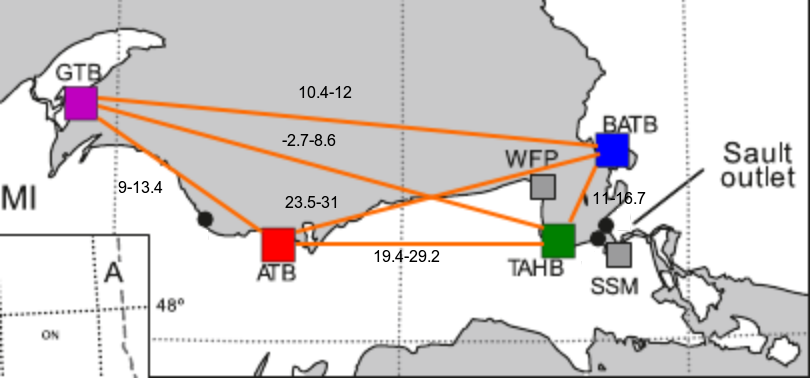
\includegraphics[width=0.72\paperwidth]{johnstonLaurentianMapWithMyGIARates.png}}
	\caption{Relative GIA Rates produced by this papers method, all values reported in cm/century}
	\label{fig:myGIARates}
\end{figure}
\newpage
\begin{figure}[h]
	\makebox[\textwidth]{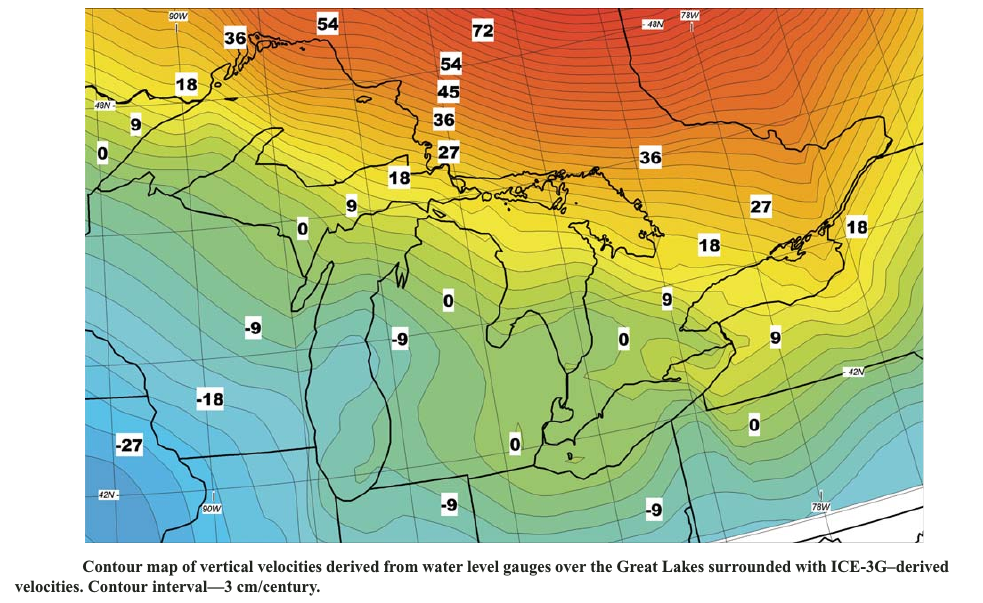
\includegraphics[width=0.72\paperwidth]{mainvilleGias.png}}
	\caption{Relative GIA Rates produced by Mainville \& Craymer, all values reported in cm/century (reproduced from Mainville \& Craymer, 2005)}
	\label{fig:craymerGIARatesBigPlot}
\end{figure}

The equivalent values for rates between sites as produced by Mainville \& Craymer
are inferred from subtracting the difference in contour between sites as shown in
Figure \ref{fig:craymerGIARatesBigPlot}, and are presented in Figure \ref{fig:craymerGIARates}.

\begin{figure}[h]
	\makebox[\textwidth]{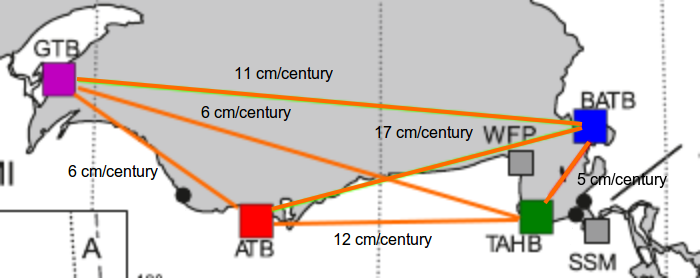
\includegraphics[width=0.72\paperwidth]{johnstonLaurentianMapWithCraymerGIARates.png}}
	\caption{Relative GIA Rates produced by Mainville \& Craymer}
	\label{fig:craymerGIARates}
\end{figure}
\newpage



The results of the analysis conducted in the previous section are summarized in
Figures 24 \& 25. Figure 24 shows confidence intervals on absolute values of
rates of GIA for each and every site comparison calculated in Section 4. Each
pair of site comparisons is grouped in vertical order in order to show how each pair
of intervals overlaps, the range of GIA values in which they overlap is used as
the estimate of the absolute value GIA rate between the given pair of sites. 
The ranges produced from this method are then printed next to a line
connecting sites in Figure 25, providing a visualization of the findings of this 
paper. A similar figure is compiled in Figure 27, summarizing the same findings
as reported by Mainville \& Craymer.

Comparing this papers results with those of Mainville \& Craymer, the value of
GIA reported by Mainville \& Craymer fell within the range reported by this paper
for 2 of the 6 pairs of sites (GTB \& TAHB and GTB \& BATB). For the remaining
four pairs of sites, the 95p confidence intervals on GIA calculated by this paper
tended to be larger than the equivalent values in Mainville \& Craymer, 
(namely ATB \& BATB, GTB \& ATB, and TAHB \& BATB) and sometimes much larger
(such as between ATB \& TAHB).

Given that the results of this paper are all on the same order of magnitude with
those reported by Mainville \& Craymer using data over a much shorter timescale,
this papers method can be inferred to be reasonably effective, but the
differences do need to be considered. These discrepancies may be an indication 
that the process of GIA in the LGL region behaved differently in the past than
in the more recent sample of time looked at by Mainville \& Craymer. One
particular area where significant
disagreement occurs is between sites ATB, BATB, and TAHB, especially in the much
larger values produced by this paper between ATB-BATB and ATB-TAHB. Given that both
of these site combinations are separated by an East-West line, this could imply
that the location of the center of the Laurentide Ice Sheet during the last glaciation being to the
north and west of Lake Superior had a stronger effect on the overall process of
rebound than the simple fact that areas to the north were more likely to be
depressed by the weight of ice sheets than areas further south. 

This interpretation should be taken with caution, given that the values produced
by this paper
may also be affected by differing quality of each intra-site measurement. Quality
of each GIA measurement is a subjective property, but it can be inferred that comparisons
that use as many data points as possible, which are evenly spread across as many 
200 year bins as possible, and have even quality between forward 
and reverse comparisons are more trustworthy than those that fail one or more of
those criteria. With that in mind, in the opinion of the Author of this paper,
the comparisons between GTB \& TAHB, GTB \& BATB, and TAHB \& ATB are of lesser
quality relative to the others. Coincidentally, two of these three comparisons
are those that agreed with Mainville \& Craymer, being lower in relative terms than
the rest of the comparisons. This could be interpreted to mean that the process of
GIA occurred at a higher rate over the longer periods of time studied by the
method of Johnston et al (2012) than it did over the shorter (and more recent)
span of time studied by that of Mainville \& Craymer (2005). Ultimately, this
conclusion is still an interpretation however, and the best method of determining
whether discrepancies between this papers method and previous ones would be to 
repeat the process with a dataset with better data coverage. One possible method
of accomplishing this would be further collection of data from sites already studied
in Johnston et al (2012), and by combining the data gathered from strandplains
closely spaced together around the lake basin.
